\documentclass[a4paper,twoside,11pt, fleqn]{article}
\usepackage{a4wide,graphicx,fancyhdr,amsmath,amssymb}
\usepackage{listings}
\usepackage{color}
\usepackage{dirtree}

%----------------------- Macros and Definitions --------------------------

\setlength\headheight{20pt}
\addtolength\topmargin{-10pt}
\addtolength\footskip{20pt}

\newcommand{\N}{\mathbb{N}}
\newcommand{\ch}{\mathcal{CH}}

\newcommand{\solution}[1]{\noindent{\bf Solution to Exercise #1:}}

\fancypagestyle{plain}{%
\fancyhf{}
\fancyhead[LO,RE]{\sffamily\bfseries\large technische universiteit eindhoven}
\fancyhead[RO,LE]{\sffamily\bfseries\large 2IN35 VLSI}
\fancyfoot[LO,RE]{\sffamily\bfseries\large department of mathematics and computer science}
\fancyfoot[RO,LE]{\sffamily\bfseries\thepage}
\renewcommand{\headrulewidth}{0pt}
\renewcommand{\footrulewidth}{0pt}
}

\pagestyle{fancy}
\fancyhf{}
\fancyhead[RO,LE]{\sffamily\bfseries\large technische universiteit eindhoven}
\fancyhead[LO,RE]{\sffamily\bfseries\large 2IN35 VLSI}
\fancyfoot[LO,RE]{\sffamily\bfseries\large department of mathematics and computer science}
\fancyfoot[RO,LE]{\sffamily\bfseries\thepage}
\renewcommand{\headrulewidth}{1pt}
\renewcommand{\footrulewidth}{0pt}

\def\addsquare#1{\tikz\node[draw]{#1};} 

%-------------------------------- Title ----------------------------------

\title{\vspace{-\baselineskip}\sffamily\bfseries Assignment 3}
\author{
	Rick Veens \qquad Studentno: 0912292\\
	\texttt{r.veens@student.tue.nl}
	\and
	Barry de Bruin \qquad Studentno: -\\
	\texttt{-@student.tue.nl}
}

\date{\today}

\setlength\parindent{0pt}

%--------------------------------- Text ----------------------------------

\begin{document}
\maketitle
\newpage

\section{Lab assignment 3a}

\subsection{Requirements}
\label{sec:req3a}

The assignment is to design and implement a FIR filter named filter that:
\begin{enumerate}
\item Uses as little resources as possible and is maximally sequential. In particular at most 1
multiplier may be used.
\item Conforms to the 4-phase asynchronous protocol for both input and output.
\item Can run at a clock frequency of 100 Mhz.
\item Honors changes in the coefficients (after a finite delay).
\item May produce a finite length interval of start-up noise
\end{enumerate}

\subsubsection{Analysis of requirements}
The FIR filter should make use of only one DSP-unit, since the internal clock frequency is significantly higher than the expected sample rate. Furthermore the coefficients should not be buffered but must be connected as wires instead of buffering them in registers. This ensures that requirement 1 and 4 can be satisfied. For requirement 3, the clock frequency should be at least 100MHz, which will be checked in the post-synthesis report. Lastly, the asynchronous ack/req protocol will be used since there needs to be some synchronization between the testbench (44.1KHz sample rate) and the filter (100MHz sample rate).


\subsection{System architecture}
Figure one shows the global architecture of the FIR filter. 
\begin{figure}[h]
	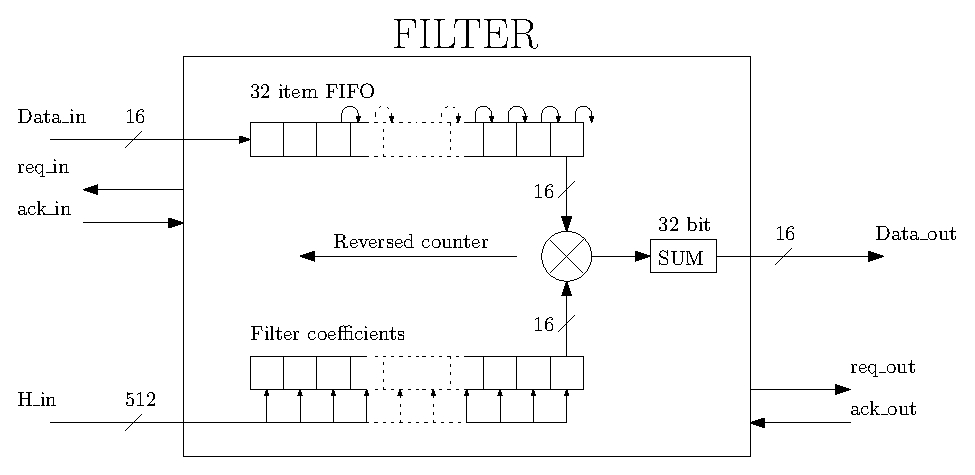
\includegraphics[scale = 1]{Images/3a_blockdiagram}
    \caption{System overview}
\end{figure}

Unlike the FIR filter of lab2, the filter has only one tap. After each clock edge the multiplier/accumulator will multiply a sample that is stored in the memory with it's corresponding filter coefficient. An index makes sure that this operation moves through the FIFO in 32 clock cycles. The index sample is also shifted one place to the right. After 32 cycles the last tap has  been calculated and the first place in the FIFO is empty. The system will output the calculated sample, and request a new data item, which will be put on the first index.\\ 

The whole procedure will then restart.
\subsection{Design choices}
We made the following design choices in filter.v (this is the only relevant file):
\begin{itemize}
	\item Added busy state \textit{state\_busy} to filter.v.
		\subitem This is used to create time for the sequential equation. 
	\item Added a counter variable \textit{cnt} that loops from 31 downwards to 0. It is set back to 31 when a new tap gets calculated.
	\item Added buffer \textit{mem} that buffers the input (size: input * 32)
		\subitem On every clock each position in the memory gets shifted to the next.
	\item Input coefficient wires (h\_in) are being split into an array of wires called \textit{coef}. \\ \textit{coef} ranges from 0 to 31.
		\subitem This enables us to easily index into the filter coefficients.
	\item Added sum register for storing intermediate tap calculations.
		\subitem We make use of the \textit{cnt} counter to index into \textit{coef}
	\item Added output buffer register to improve the throughput to a steady 100MHz.

\end{itemize}


\subsection{Functional correctness}
Also see section~\ref{sec:req3a} for a list of the requirements.
\begin{enumerate}
	\item The implementation of the FIR filter uses only 1 DSP unit. See the				section~\ref{sec:resc3a} for more details about resources used by 		the implementation.
	\item Please refer to section~\ref{code:3a}, starting from line 47 for our implementation of the busy state of the filter.
	\item See section~\ref{sec:3athrolat} for an analysis of timing results. Note that the throughput is above 100MHz.
	\item The wires of input $h\_in$ (size CWIDTH) are separated into a verilog 			array of wires with a generate block during synthesis. 
	
	Meaning that not the coefficients are saved but just the wires of $h\_in$ are used. If any of the input coefficients were to change during the execution of the filter, after at most 32 taps the new coefficients will be correctly used.
	\item This requirement was already met with the unmodified exercise-code.
\end{enumerate}

\subsection{Resource usage}
\label{sec:resc3a}

Table~\ref{tab:3ausage} summarizes the resources used by the FIR filter. This list is obtained by running the synthesis step in Xilinx ISE and extracted from the \textit{Summary} and \textit{Device Utilization} report.

\begin{table}[h]
\begin{tabular}{|l|l|l|l|}
\hline
\textbf{Resource} & \textbf{Available} & \textbf{Utilized} & \textbf{Percentage utilized}\\
\hline
Flip Flops	& 54576 & 1080 	& 1\%\\
Slice LUTs 	& 27288 & 500 	& 1\%\\
DSP48A1s	& 58 	& 1 	& 1\%\\
BRAM		& 116 	& 0 	& 0\%\\
Bonded IOBs	& 218 	& 40 	& 18\%\\
\hline
\end{tabular}
\caption{General resource usage overview}
\label{tab:3ausage}
\end{table}

The number of flipflops used in the design are:
\begin{align*}
Total_{\#reg}	&= sum + output\_buf + data + coef + cnt + state + flow control\\
			&= 32 + 16 + 16\cdot 32 + 32\cdot 16 + 5 + 1 + 2\\
			&= 1080
\end{align*}
This number matches the synthesis result.\\

There is only one DSP unit used, since the filter is fully sequential. This results in a significant resource reduction since we only have 58 DSP units. According to the summary report, 365 slice LUTs are used for logical ports. They are used to model the 5 bit counter that counts up to 32. The number of Bonded IOB's represents the number of pins used on the FPGA. These pins are occupied by the clk, rst, h\_in, h\_enabled,  $2\cdot 16$ input and output pins and 2 pairs of ack/req pins.\\

Furthermore some additional resources are used to enable the possibility to shift the data in the FIFO every clock cycle.

\subsection{System throughput and latency}
\label{sec:3athrolat}
The minimum sample time estimation is extracted from the \textit{Synthesis report} under \textit{Timing Report}.\\

   \textit{Minimum period: 8.421ns (Maximum Frequency: 118.750MHz)\\
   Minimum input arrival time before clock: 6.562ns\\
   Maximum output required time after clock: 3.791ns}\\

This time is equal to the largest critical path (the calculation of the tap is the critical path in this design).\\

After doing the placement and routing step, we will get a more accurate measurement of the maximum achievable throughput. These measurements can be found in the \textit{Advanced Post-PAR static timing report} under \textit{Timing summary}:\\

\textit{Minimum period:   9.712ns\{1\}   (Maximum frequency: 102.965MHz)\\
   Minimum input required time before clock:   8.630ns\\
   Maximum output delay after clock:   8.824ns}\\

Since the minimum period is the maximum delay, we can be sure that our design is able to run at 100MHz. First we didn't buffer the output data. This did cost us a large increment in 'Maximum output delay after clock'. Therefore our design only ran at 90MHz. At a small cost of buffering the filter output, we are now able to reach 100MHz.

\subsection{Simulation results}
\begin{figure}[h]
	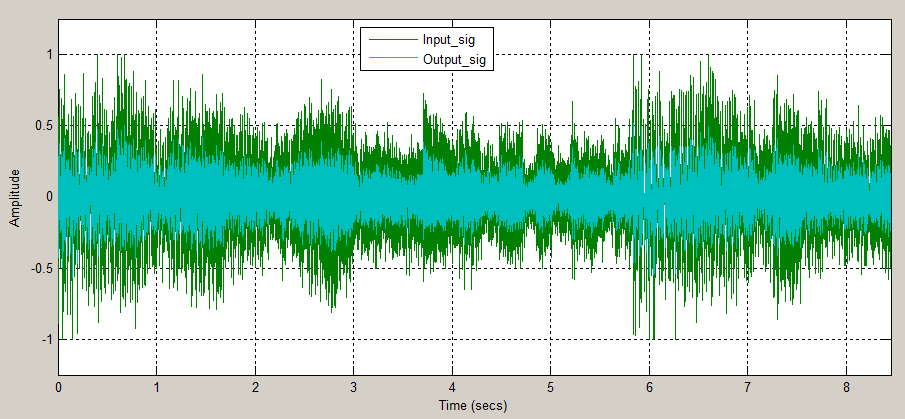
\includegraphics[scale = 0.71]{Images/3a_timedomain_inputoutput}
    \caption{Input (green) and output(blue) signal of filter}
\end{figure}

\begin{figure}[h]
	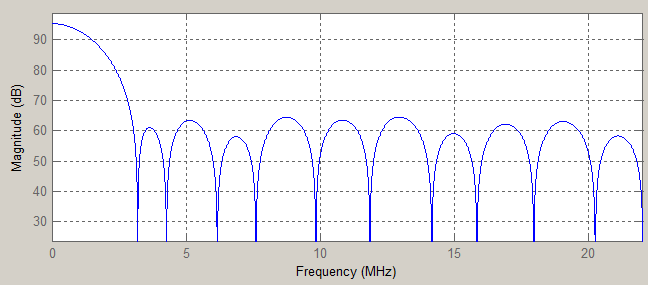
\includegraphics[scale = 1]{Images/3a_filterrespons}
    \caption{General filter response}
\end{figure}

\begin{figure}[h]
	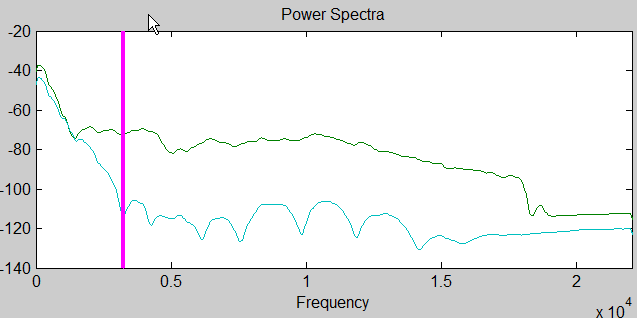
\includegraphics[scale = 1]{Images/3a_powerspectra}
    \caption{Frequency response of input(green) and output(blue)}
\end{figure}

\newpage
The results match the original filter behavior. Therefore we can say that the filter is still working correctly.


\newpage
\section{Lab assignment 3b}
\subsection{Requirements}
The specific requirements for the strength reduced FIR filter are:
\begin{enumerate}
\item The design may use at most 3 multipliers.
\item Conforms to the 4-phase asynchronous handshake protocol for both input and output.
\item Can run at a clock frequency of 100 Mhz.
\item Should have about 4 times the sample frequency as the sequential implementation.
\item Honors changes in the coefficients (after a finite delay).
\item May produce a finite length interval of start-up noise.
\end{enumerate}
\subsubsection{Analysis of requirements}
We use the strength-reduced 2-parallel implementation of Parhi. This implementation uses 3 multipliers and ensures a throughput of 4 times the standard 1 multiplier implementation. To be sure that this frequency can be achieved, we must also ensure that the filter runs on 100MHz and does not take much more than 16 (\# of stages) cycles for two 16-bit samples. Coefficients can also change during runtime. Because the filter consists of three subfilters (filter = active component), the handshake protocol is established with help of passivators.

\subsection{System architecture}
 A block diagram of parhi's filter is shown below:
 
\begin{figure}[h]
	
	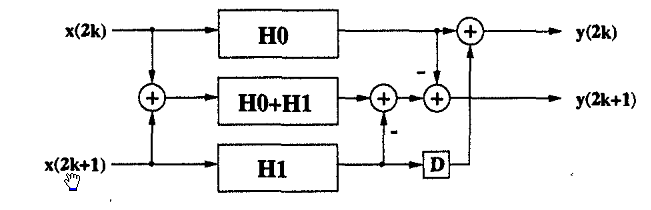
\includegraphics[scale = 0.71]{Images/3b_parhi}
    \caption{Parhi's 2-Parallel strength reduced FIR filter}
    \label{fig:3bparhi}
\end{figure}

We have decided to split the filter up in multiple parts, to make the implementation easier:
\begin{enumerate}
	\item \textit{Pre-processing} \\
		Splits the input data into the three output streams as seen on the left side of figure	\ref{fig:3bparhi}. \\
		Furthermore, the input coefficients $h\_in$ are split into the even coefficients (H0), odd coefficients (H1) and sum of the even and odd coefficients (H0+H1).

	\item \textit{Parallel filtering} \\
	The filter of assignment 3a is used in parallel to process each part of parhi's filter as shown in the middle section of figure	\ref{fig:3bparhi}.
	
	\item \textit{Post-processing} \\
	This part receives the data from the parallel filters, applies the operations shown on the right side of figure \ref{fig:3bparhi}, and delivers output.
\end{enumerate}

The hierarchy of the implementation of assignment 3b is as follows: 
\dirtree{%
.1 filter.
.2 mainfilter.
.3 preproc.
.3 subfilter (3x).
.3 passivator (6x).
.3 postproc.
}
In this hierarchy, the top level element implements the communication with the filter implementation and $filtertest$. We chose to implement a $mainfilter$ module that contains all of the wiring of the many connected modules.

Note that the $subfilter$ module is the implementation of assignment 3a, adjusted to process 16 taps instead of 32.

Figure~\ref{fig:3bblockdiag} displays the layout of the modules.
\begin{figure}[h]
	\centering
	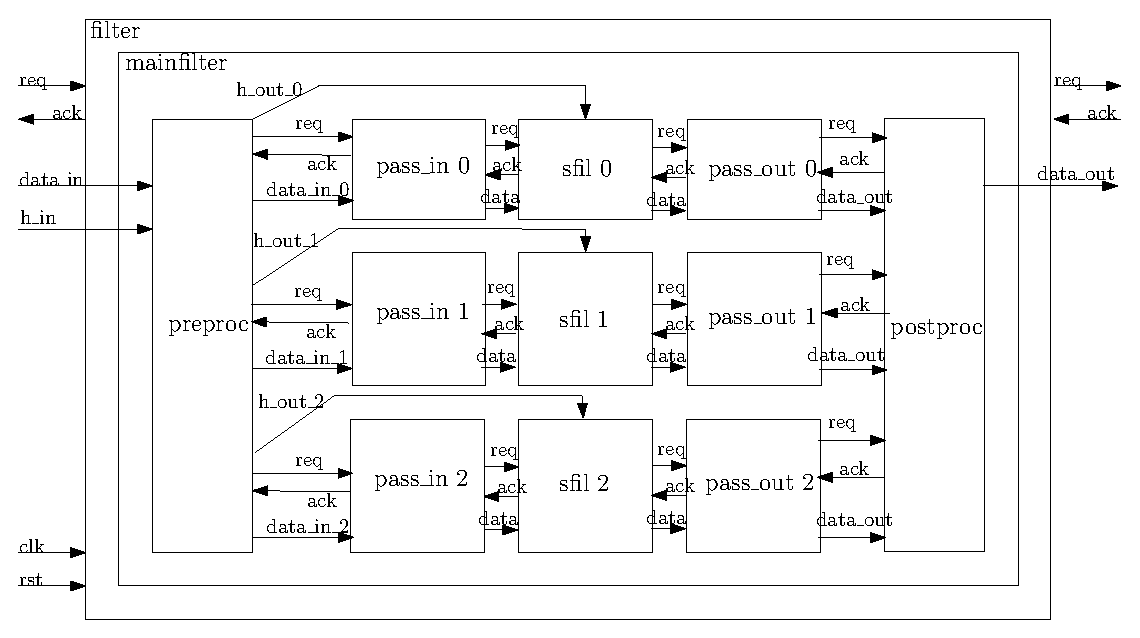
\includegraphics[scale=1.0]{./Images/3b_blockdiagram.eps}
	\caption{Block diagram of assignment 3b, with a few abstractions.}
	\label{fig:3bblockdiag}
\end{figure}

\subsection{Design choices}
\subsection{Functional correctness}
\subsection{Resource usage}
Table~\ref{tab:3busage} summarizes the resources used by the FIR filter. This list is obtained by running the synthesis step in Xilinx ISE and extracted from the \textit{Summary} and \textit{Device Utilization} report.

\begin{table}[h]
\begin{tabular}{|l|l|l|l|}
\hline
\textbf{Resource} & \textbf{Available} & \textbf{Utilized} & \textbf{Percentage utilized}\\
\hline
Flip Flops	& 54576 & 2471 	& 4 \%\\
Slice LUTs 	& 27288 & 804 	& 2 \%\\
DSP48A1s	& 58 	& 3 	& 5 \%\\
BRAM		& 116 	& 0 	& 0 \%\\
Bonded IOBs	& 218 	& 72 	& 33 \%\\
\hline
\end{tabular}
\caption{General resource usage overview}
\label{tab:3busage}
\end{table}

The amount of registers in assignment 3b compared to assignment 3a have increased from 1080 to 2471. This is an increase of 128\%. 

In this version the sequential filter computes 16 instead of 32 taps but in parallel of three. So we could say $(1080/2)*3=1620$. We have around 800 missing registers. These additional registers can be explained as being the result of numerous pipelining.

\smallskip

There are 2 additional DSP units utilized, this is because of the triple pipelining of the sequential filter of assignment 3a.

There is no blockram used, no change compared to assignment 3a.

Furthermore, the Boned IOBs have increase by 32 because testbench now send/receives DDWIDTH instead of DWIDTH from the filter.

\subsection{System throughput and latency}
The minimum sample time estimation is extracted from the \textit{Synthesis report} under \textit{Timing Report}.\\

   \textit{Minimum period:  7.256ns (Maximum Frequency: 137.820MHz)\\
   Minimum input arrival time before clock: 6.449ns\\
   Maximum output required time after clock: 3.701ns}\\

This time is equal to the largest critical path (the calculation of the tap is the critical path in this design).\\

After doing the placement and routing step, we will get a more accurate measurement of the maximum achievable throughput. These measurements can be found in the \textit{Advanced Post-PAR static timing report} under \textit{Timing summary}:\\

\textit{Minimum period:   8.164ns\{1\}   (Maximum frequency: 122.489MHz)\\
   Minimum input required time before clock:   9.259ns\\
   Maximum output delay after clock:   8.647ns}\\

Since the minimum period is the maximum delay, we can be sure that our design is able to run at 100MHz.

\subsection{Simulation results}



\newpage
\section{Comparison between two filters}
In your final report, compare the output signals of the strength reduced filter with the output of the sequential filter, by generating a difference signal for a representative subset of
samples. Make sure you align the outputs correctly, because the amount of start-up noise of
the 2 implementations may differ. If the difference signal is non-zero, explain the differences.
Further reporting guidelines are on the course’s website.

\newpage
\section{Appendix: code listings}

\subsection{Assignment 3a code}
\label{code:3a}

\lstset{ %
	numbers=left
}

\begin{lstlisting}[language=Verilog]
`timescale 1ns / 1ps

module filter #(parameter NR_STAGES = 32,
                parameter DWIDTH = 16,
                parameter DDWIDTH = 2*DWIDTH,
                parameter CWIDTH = NR_STAGES * DWIDTH)
  (input  clk,
   input  rst,
   output req_in,
   input  ack_in,
   input signed [0:DWIDTH-1] data_in,
   output req_out,
   input  ack_out,
   output signed [0:DWIDTH-1] data_out,
   input signed [0:CWIDTH-1] h_in);

  // Output request register
  reg req_out_buf;
  assign req_out = req_out_buf;

  // Input request register
  reg req_in_buf;
  assign req_in = req_in_buf;

  // Accumulator (Buffer output to decrease 'Maximum output delay after clock')
  reg signed [0:DDWIDTH-1] sum;
  reg signed [0:DWIDTH-1] data_out_buf;
  assign data_out = data_out_buf; 

  // Memory to store last 32 inputs and memory to store the coefficients.
  reg signed [0:DWIDTH-1] mem[0:NR_STAGES-1];
  wire signed [0:DWIDTH-1] coef[0:NR_STAGES-1];

  // State variables for FIR
  reg state_busy;
  reg [4:0] cnt;

  // Split the coefficient into 32 wire busses of 16 bit
  generate
    genvar i;
    for (i = 0; i < NR_STAGES; i = i +1)begin : coef_split
      assign coef[i] = h_in[i*DWIDTH +: DWIDTH];
    end
  endgenerate

  // State machine that controls the flow control between testbench and filter
  always @(posedge clk) begin
    if (rst) begin
      state_busy <= 0;
      req_in_buf <= 0;
      req_out_buf <= 0;
      sum <= 0;
      cnt <= NR_STAGES-1;
    end
    else begin
      // Request for input sample is acknowledged. Start calculating
      if (req_in && ack_in) begin
        mem[0] <= data_in;
        state_busy <= 1;
        req_in_buf <= 0;
      end

      // Process the output in 32 cycles. Then initiate a req_out to warn the output that a sample is ready
      if (state_busy && !req_out) begin
        // Shift through the data and calculate one tap every clock cycle
        mem[cnt+1] <= mem[cnt];
        sum <= sum + mem[cnt]*coef[cnt];
        cnt <= cnt - 1;

        // When a complete cycle is done (32 taps calculated), start to output the outcome
        if(cnt == 0) begin
          data_out_buf <= sum[0:15];
          req_out_buf <= 1;
        end
      end

      // If req_out is acknowledged, reset all variables
      if (req_out && ack_out) begin
        req_out_buf <= 0;
        state_busy <= 0;
        sum <= 0;
      end

      // Wait until everyone is calmed down, then initiate new sample request
      if (!req_in && !req_out && !ack_in && !ack_out && !state_busy) begin   
        req_in_buf <= 1;
      end	
    end
  end

endmodule
\end{lstlisting}

\end{document}
